%%%%%%%%%%%%%%%%%%%%%%%%%%%%%%%%%%%%%%%%%%%%%%%%%%%%%%%%%%%%%%%%%%%%%%%%%%%%%%%%
% Talk: segmentation under fragmented occlusion (NFO-VOS, Layer-SAM). 16:9 TUM template (Vorlagen/Praesentation16zu9.tex).
% Compile from this directory:  latexmk -pdf NFO_VOS_talk
% Slides carry keywords only; what to say is in \note{} (hidden; to see the notes, uncomment the pgfpages lines below).
% Numbers: 32 whole crossings unless a note says otherwise (docs/vos_benchmark/nfo_vos_pilot_findings.md §9);
% annotator B (seq2, seq3, 15 frames): data/nfo_processed/seq*_gt/*_handAv_annot2.png.
% \Platzhalter{w}{h}{what}: an image still to be chosen. Figures: plots/nfo/ (poster), plots/talk/ (talk only;
% benchmark/nfo_vos/tools/talk_figures.py). Earlier versions: NFO_VOS_talk_draft.tex (poster turned into slides).
%
% Story: SVOS, masks, PVS -> fragmented occlusion (never a full view) -> hard, humans disagree -> modal, keep the
% evidence -> what can go wrong with PVS -> NFO-VOS (start positions, three scores, integral image in detection)
% -> memory vs where (trade-off) -> motion layers -> tracker -> two layers -> Layer-SAM (evidence, not memory) -> adapter,
% synthetic data, loss -> results -> conclusion.
%%%%%%%%%%%%%%%%%%%%%%%%%%%%%%%%%%%%%%%%%%%%%%%%%%%%%%%%%%%%%%%%%%%%%%%%%%%%%%%%

\PassOptionsToPackage{english,ngerman}{babel} % English hyphenation, selected after \begin{document}
\input{./Ressourcen/Praesentation/Praeambel16zu9.tex} % Seitenverhältnis 16:9
\input{./_Einstellungen.tex}                    % !!! DATEI ANPASSEN !!!

\usepackage{amssymb} % \checkmark
\usetikzlibrary{arrows.meta,positioning,calc,fit,backgrounds,shapes.geometric}
% speaker notes on a second screen:
% \usepackage{pgfpages}\setbeameroption{show notes on second screen=right}

\renewcommand{\PersonTitel}{}
\renewcommand{\PersonVorname}{Ido}
\renewcommand{\PersonNachname}{Akov}
\renewcommand{\LehrstuhlName}{Computer Vision Group}
\renewcommand{\PraesentationFusszeileZusatz}{}

\title{Seeing through Foliage}
\newcommand{\Untertitel}{Video object segmentation under natural fragmented occlusion}
\author{{\PraesentationSchriftgroesseGross\selectfont\Untertitel}\\[8mm]Ido Akov}
\institute[]{Computer Vision Group, TUM\\Data Science and Artificial Intelligence (DSS-DSAI), AIT}
\date{}
\subject{Video object segmentation under fragmented occlusion}

\input{./Ressourcen/Praesentation/Anfang.tex} % !!! NICHT ENTFERNEN !!!

\selectlanguage{english}

\definecolor{ColOurs}{HTML}{2A78D6}
\definecolor{ColSamurai}{HTML}{EB6834}
\definecolor{ColBox}{HTML}{EAF1FA}
\definecolor{UniversitaetFarbe}{RGB}{0,101,189}
\newcommand{\Merke}[1]{%
  \par\noindent\colorbox{ColBox}{\parbox{\dimexpr\linewidth-2\fboxsep}{\vspace{0.2em}%
    \raggedright\color{UniversitaetFarbe}\bfseries #1\vspace{0.2em}}}\par}
\newcommand{\Klein}[1]{{\PraesentationSchriftgroesseKlein\selectfont\color{black!70}#1}}
\newcommand{\Quelle}[1]{{\PraesentationSchriftgroesseKlein\selectfont\color{black!55}[#1]}}
\newcommand{\Platzhalter}[3]{\fcolorbox{black!35}{black!4}{\parbox[c][#2][c]{#1}{\centering
  \PraesentationSchriftgroesseKlein\selectfont\color{black!55}\textbf{image}\\[1mm]#3}}}
\newcommand{\Teil}[1]{\renewcommand{\PraesentationFusszeileZusatz}{| #1}}

% \Fire / \Ice come from the poster's architecture figure, typeset once (and discarded) at top level
\newsavebox{\ArchBox}\sbox{\ArchBox}{% Our architecture in the visual language of the SAM2 paper figure (plots/nfo/model_diagram.png):
% green = image encoder, orange = mask decoder, lavender = prompt encoder, pink = memory (not used).
% Blue outline = trained by us. Natural width ≈ 20 cm; the poster scales it to the column width.
\providecommand{\ArchSub}{\fontsize{14}{16}\selectfont}
% trained (flame) / frozen (snowflake) markers, drawn so they work with pdfLaTeX and XeTeX alike
\newsavebox{\FireBox}\newsavebox{\IceBox}
\sbox{\FireBox}{\tikz[baseline=-0.1em, x=0.9em, y=0.9em]{%
  \fill[orange!90!red] (0,-0.5) .. controls (-0.55,-0.25) and (-0.35,0.25) .. (0,0.75)
                       .. controls (0.35,0.25) and (0.55,-0.25) .. (0,-0.5);
  \fill[yellow!85!orange] (0,-0.45) .. controls (-0.25,-0.25) and (-0.15,0.05) .. (0,0.25)
                          .. controls (0.15,0.05) and (0.25,-0.25) .. (0,-0.45);}}
\sbox{\IceBox}{\tikz[baseline=-0.1em, x=0.9em, y=0.9em, line width=0.12em, cyan!60!blue, line cap=round]{%
  \foreach \a in {0,60,120} {\draw (\a:-0.55) -- (\a:0.55);
    \draw (\a:0.32) -- ++(\a+35:0.18); \draw (\a:0.32) -- ++(\a-35:0.18);
    \draw (\a:-0.32) -- ++(\a+215:0.18); \draw (\a:-0.32) -- ++(\a+145:0.18);}}}
\providecommand{\Fire}{\usebox{\FireBox}}\providecommand{\Ice}{\usebox{\IceBox}}
\definecolor{SamEnc}{HTML}{D4F5C4}\definecolor{SamEncD}{HTML}{8FCF79}
\definecolor{SamDec}{HTML}{FDE6C8}\definecolor{SamDecD}{HTML}{E9B676}
\definecolor{SamPrm}{HTML}{DEDDFB}\definecolor{SamPrmD}{HTML}{9E9BE6}
\definecolor{SamMem}{HTML}{F9DDF0}\definecolor{SamMemD}{HTML}{E7A9D3}
\begin{tikzpicture}[x=1cm, y=1cm, font=\fontsize{19}{22}\selectfont,
    lab/.style={align=center, font=\fontsize{17}{20}\selectfont},
    small/.style={align=center, font=\fontsize{14}{16}\selectfont, text=black!70},
    blk/.style={rounded corners=7pt, line width=1.4pt, align=center, minimum height=1.9cm},
    ours/.style={blk, draw=ColOurs, fill=ColOurs!14, line width=2.6pt},
    stride/.style={draw=ColOurs, fill=white, rounded corners=4pt, line width=1.2pt, minimum width=2.3cm,
                   minimum height=1.1cm, font=\fontsize{15}{17}\selectfont},
    arr/.style={-{Latex[length=4mm, width=3mm]}, line width=1.8pt, draw=black!80},
    thin/.style={-{Latex[length=3mm, width=2.4mm]}, line width=1.2pt, draw=ColOurs},
    feat/.style={draw=SamEncD, fill=SamEnc!70, line width=1.1pt, minimum width=1.3cm, minimum height=1.3cm}]

  % inputs
  \node[inner sep=0pt] (X) at (-6, 0) {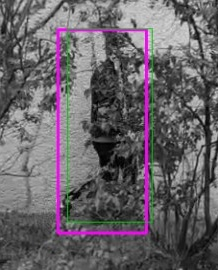
\includegraphics[height=4.2cm]{plots/nfo/inputs_0.jpg}};
  \node[inner sep=0pt] (C) at ( 0, 0) {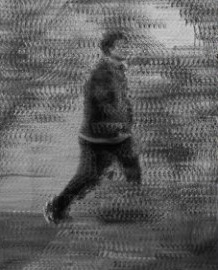
\includegraphics[height=4.2cm]{plots/nfo/inputs_2.jpg}};
  \node[inner sep=0pt] (B) at ( 6, 0) {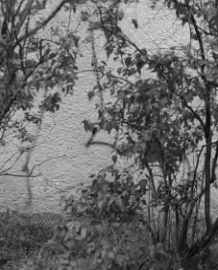
\includegraphics[height=4.2cm]{plots/nfo/inputs_1.jpg}};
  \node[lab, above=1mm of X] {\textbf{frame} $t$\\[-1mm]{\ArchSub with tracker box}};
  \node[lab, above=1mm of C] {\textbf{integral image}\\[-1mm]{\ArchSub 6 past frames, aligned}};
  \node[lab, above=1mm of B] {\textbf{empty scene}\\[-1mm]{\ArchSub encoded once per scene}};

  % shared image encoder (trapezoid, as in SAM2)
  \node[trapezium, trapezium angle=78, shape border rotate=180, draw=SamEncD, fill=SamEnc, line width=1.4pt,
        minimum width=18.5cm, minimum height=2cm, align=center] (enc) at (0, -3.9)
        {\Ice\ \textbf{image encoder}\\[-1mm]{\ArchSub same weights for all three}};
  \foreach \n/\x in {X/-6, C/0, B/6} \draw[arr] (\n.south) -- (\x, -2.9);

  % feature maps (strides 16 / 8 / 4)
  \foreach \n/\x/\t in {fx/-6/t, fc/0/I, fb/6/E} {
    \node[feat] at (\x+0.25, -6.5+0.25) {};
    \node[feat] (\n) at (\x, -6.5) {$F_{\t}$};
    \draw[arr] (\x, -4.9) -- (\n.north);
  }
  \node[small, anchor=west] at (7.0, -7.45) {strides\\16, 8, 4};

  % adapter: takes only the three feature maps; per stride, coarse to fine
  \node[ours, minimum width=15cm, minimum height=3.6cm] (ad) at (1, -9.9) {};
  \node[anchor=north west, align=left] at ([xshift=3mm, yshift=-2mm]ad.north west)
        {\Fire\ \textbf{adapter}\ \ {\ArchSub 0.7\,M parameters}};
  \node[stride] (s16) at (-3.2, -10.6) {stride 16};
  \node[stride] (s8)  at ( 0.9, -10.6) {stride 8};
  \node[stride] (s4)  at ( 5.0, -10.6) {stride 4};
  \draw[thin] (s16) -- (s8); \draw[thin] (s8) -- (s4);
  \foreach \n in {fx, fc, fb} \draw[arr] (\n.south) -- (\n.south |- ad.north);

  % corrections added to the frame features at each stride
  \node[circle, draw=black!80, line width=1.8pt, minimum size=1cm, inner sep=0pt,
        font=\fontsize{28}{28}\selectfont\bfseries] (plus) at (-9.6, -9.9) {$+$};
  \draw[arr] (fx.west) -| (plus.north);
  \draw[arr] (ad.west) -- node[above, small] {corrections} (plus.east);

  % decoder + prompt encoder
  \node[blk, draw=SamDecD, fill=SamDec, minimum width=7.2cm] (dec) at (-4.6, -13.6)
        {\Ice\ \textbf{mask decoder}};
  \node[blk, draw=SamPrmD, fill=SamPrm, minimum width=6.4cm] (pe) at (5, -13.6)
        {\Ice\ \textbf{prompt encoder}};
  \draw[arr] (plus.south) |- (dec.west);
  \draw[arr] (pe.west) -- (dec.east);
  \draw[arr, dashed] (pe.north |- ad.south) -- node[right, small] {point\\[-1mm]correction} (pe.north);

  % tracker: where to look
  \node[blk, draw=ColOurs, fill=white, line width=1.4pt, minimum width=6.4cm] (trk) at (5, -16.5)
        {\textbf{tracker}\\[-1mm]{\ArchSub motion + box: where to look}};
  \draw[arr] (trk.north) -- (pe.south);
  % tracker input: change of the frame features against the empty scene
  \draw[-{Latex[length=3mm, width=2.4mm]}, line width=1.2pt, draw=black!60] (fb.east) -- (9.2, -6.5) -- (9.2, -15.9)
        node[pos=0.5, rotate=-90, anchor=south, inner sep=1.5pt, small] {change of $F_t$ vs $F_E$} -- ([yshift=6mm]trk.east);
  % the tracker's motion builds the integral image
  \draw[arr, draw=ColOurs, dashed] (trk.east) -- ++(1.6, 0) |- ([yshift=3.4cm]C.north) node[pos=0.75, above, small, text=ColOurs]
        {motion: aligns the past frames} -- ([yshift=1.75cm]C.north);
  % legend
  \node[anchor=south west, align=left, font=\fontsize{16}{19}\selectfont] at (-11.6, -21.4)
        {\Fire\ trained (ours)\\ \Ice\ frozen SAM2.1};

  % output
  \node[inner sep=0pt] (M) at (-4.6, -18.1) {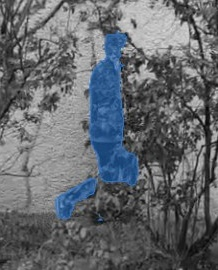
\includegraphics[height=4.2cm]{plots/nfo/inputs_6.jpg}};
  \draw[arr] (dec.south) -- (M.north);
  \node[lab, left=2mm of M] {\textbf{mask}};

  % memory path of SAM2: not used
  \node[blk, draw=SamMemD, fill=SamMem!50, dashed, minimum width=6.4cm, text=black!55] (mem) at (5, -19.4)
        {memory of past masks\\[-1mm]{\ArchSub not used}};
  \draw[arr, draw=black!35, dashed] (M.east |- mem.west) -- node[text=ColSamurai, font=\fontsize{30}{30}\selectfont\bfseries]
        {$\times$} (mem.west);
\end{tikzpicture}
%
  \global\setbox\FireBox\copy\FireBox\global\setbox\IceBox\copy\IceBox\global\let\Fire\Fire\global\let\Ice\Ice}

\tikzset{
  box/.style={draw=black!70, rounded corners=3pt, line width=0.8pt, align=center, minimum height=9mm, inner sep=4pt},
  dec/.style={box, draw=ColSamurai, fill=ColSamurai!12},
  info/.style={box, draw=ColOurs, fill=ColOurs!12},
  sam/.style={box, fill=black!5},
  ar/.style={-{Latex[length=2.6mm]}, line width=0.9pt},
}

% the scene seen from the side: camera, foliage in front, person, background behind.
% #1 = 1: with each layer's velocity (static camera)
\newcommand{\Schichten}[1]{%
\begin{tikzpicture}[x=1cm, y=1cm]
  \fill[black!70] (0, 1.6) -- (0.7, 1.95) -- (0.7, 1.25) -- cycle; \fill[black!70] (-0.5, 1.3) rectangle (0, 1.9);
  \node[below, font=\PraesentationSchriftgroesseKlein\selectfont] at (0, 1.2) {camera};
  \foreach \x/\c/\l/\v in {2.2/TUMGruen!70/foliage/{$v \approx 0$}, 4.6/black!55/person/{$v$}, 7.0/black!30/background/{$v = 0$}} {
    \fill[\c, opacity=0.85] (\x, 0) -- (\x + 0.9, 0.7) -- (\x + 0.9, 3.9) -- (\x, 3.2) -- cycle;
    \node[below, font=\PraesentationSchriftgroesseKlein\selectfont] at (\x + 0.45, -0.05) {\textbf{\l}};
    \ifnum#1=1 \node[below, font=\PraesentationSchriftgroesseKlein\selectfont] at (\x + 0.45, -0.55) {\v}; \fi
  }
  \draw[dashed, black!40] (0.7, 1.6) -- (7.9, 2.3);
\end{tikzpicture}}


\PraesentationMasterStandard
\PraesentationTitelseite

%=========================================================================================== I. VOS, PVS
\Teil{Segmenting objects in video}

\begin{frame}
\frametitle{Semi-supervised video object segmentation (SVOS)}
\centering\includegraphics[width=0.74\textwidth]{plots/talk/DAVIS-VOS.png}

\medskip
given: the object's mask in frame $t_0$ \quad$\longrightarrow$\quad wanted: its mask in every later frame\\
\Quelle{DAVIS: Perazzi et al.\ 2016}
\note[itemize]{
\item SVOS: give the object's mask (or box, or clicks) in the first frame; the model keeps segmenting it in every later frame, with one consistent identity.
\item Any object, not a fixed set of classes. Benchmarks: DAVIS, YouTube-VOS, MOSE, LVOS.
\item A mask, not a box: a box says where the object is, a mask says which pixels belong to it.
\item Image source: to fill in.
}
\end{frame}

\begin{frame}
\frametitle{Prompted video segmentation (PVS)}
\centering\includegraphics[width=0.86\textwidth]{plots/nfo/model_diagram.png}\\
\Quelle{figure: SAM 2, Ravi et al.\ 2024}

\medskip
\raggedright
\begin{itemize}
\item one prompt (box + point) $\to$ masks for the whole video
\item SAM2: a \textbf{memory} of its own past masks; SAMURAI manages it better
\end{itemize}
\Quelle{SAMURAI: Yang et al.\ 2024}
\note[itemize]{
\item Dense masks by hand cost minutes per frame. A promptable model turns one cheap prompt into masks for the whole video; this is now how dense labels are made (SAM2's own data engine).
\item SAM2: image encoder, prompt encoder, mask decoder, and a memory bank of past frame features fused with SAM2's own past masks. Every frame attends to that memory.
\item SAMURAI (Kalman motion to pick memories); also SAM2Long, DAM4SAM: all improve \emph{which} past decisions to keep. SAMURAI is our baseline throughout.
\item Question for the rest of the talk: what happens to this design when the object is behind foliage?
}
\end{frame}

%=========================================================================================== II. fragmented occlusion
\Teil{Fragmented occlusion}

\begin{frame}
\frametitle{Fragmented occlusion}
\centering\only<1>{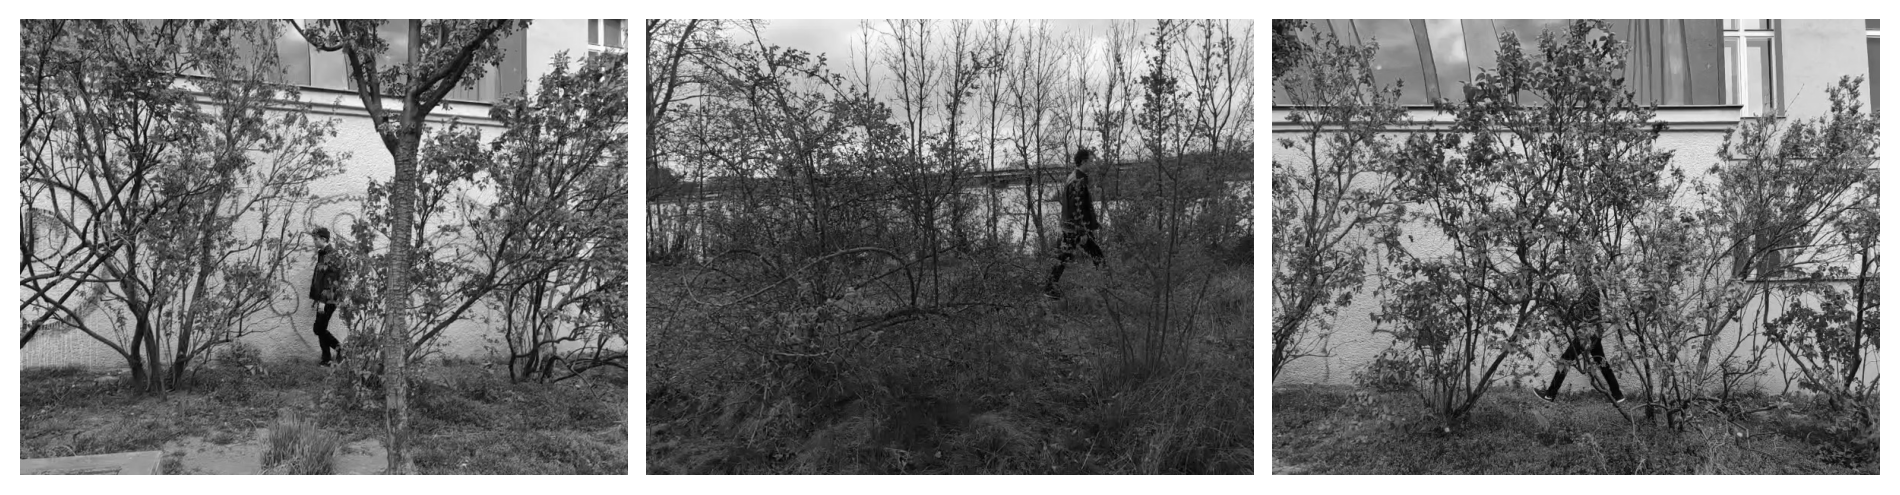
\includegraphics[width=0.96\textwidth]{plots/talk/scenes_nobox.png}}%
\only<2>{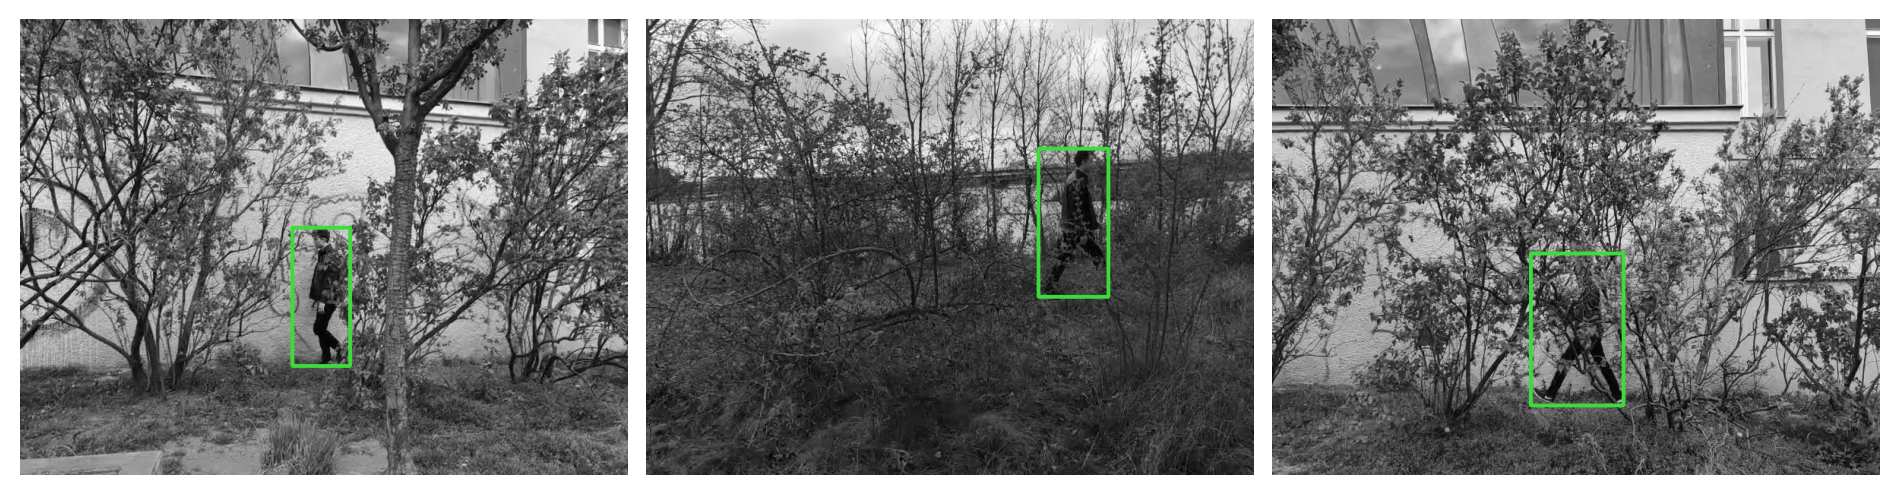
\includegraphics[width=0.96\textwidth]{plots/talk/scenes.png}}

\medskip\raggedright
\only<1>{\textbf{Where is the person?}}%
\only<2>{%
\begin{itemize}
\item partial occlusion: one occluder hides a part
\item full occlusion: the object disappears and returns
\item fragmented: a wall of leaves, \textbf{never a full view}
\end{itemize}}
\note[itemize]{
\item First ask the room to find the person in each frame; then reveal.
\item SVOS models are trained for partial and full occlusion. Both assume the object was seen clearly at some point, typically at the prompt, and memory holds that view.
\item Under fragmented occlusion that view never exists. Hand labels: in the median frame about 60\,\% of the body is visible, always in pieces.
\item Where it matters: surveillance at forest edges, search and rescue under canopy, wildlife cameras, fences and blinds.
}
\end{frame}

\begin{frame}
\frametitle{Why fragmented occlusion is hard}
\vspace*{2mm}
\begin{columns}[T]
\begin{column}{0.46\textwidth}
\centering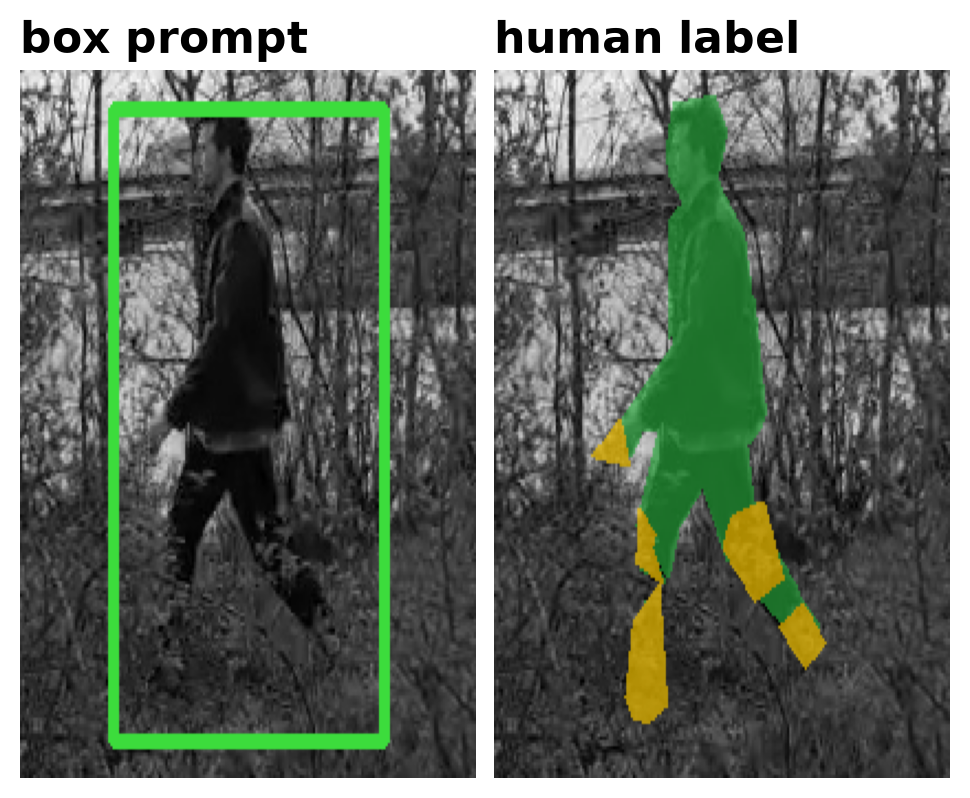
\includegraphics[height=6.6cm]{plots/talk/prompt.png}
\end{column}
\begin{column}{0.52\textwidth}
\begin{itemize}
\item fragments can be arbitrarily small
\item leaves move, light changes; grayscale
\item a perfect box still holds mostly foliage
\item some pixels mix person and leaf: \textbf{ambiguous} \textcolor[RGB]{230,184,0}{$\blacksquare$}
\end{itemize}
\end{column}
\end{columns}
\note[itemize]{
\item Say: even with a perfect prompt, segmentation is uncertain.
\item Fragments can be as small as a pixel; a segmentation network decides on a coarse grid and bridges or drops them.
\item Left: the hand-drawn box and the human label of the same frame. Green: person. Yellow: the annotator could not decide (here: the legs behind twigs). This colour code holds for the whole talk.
}
\end{frame}

\begin{frame}
\frametitle{Annotator agreement}
\centering
\vspace*{1mm}
\only<1>{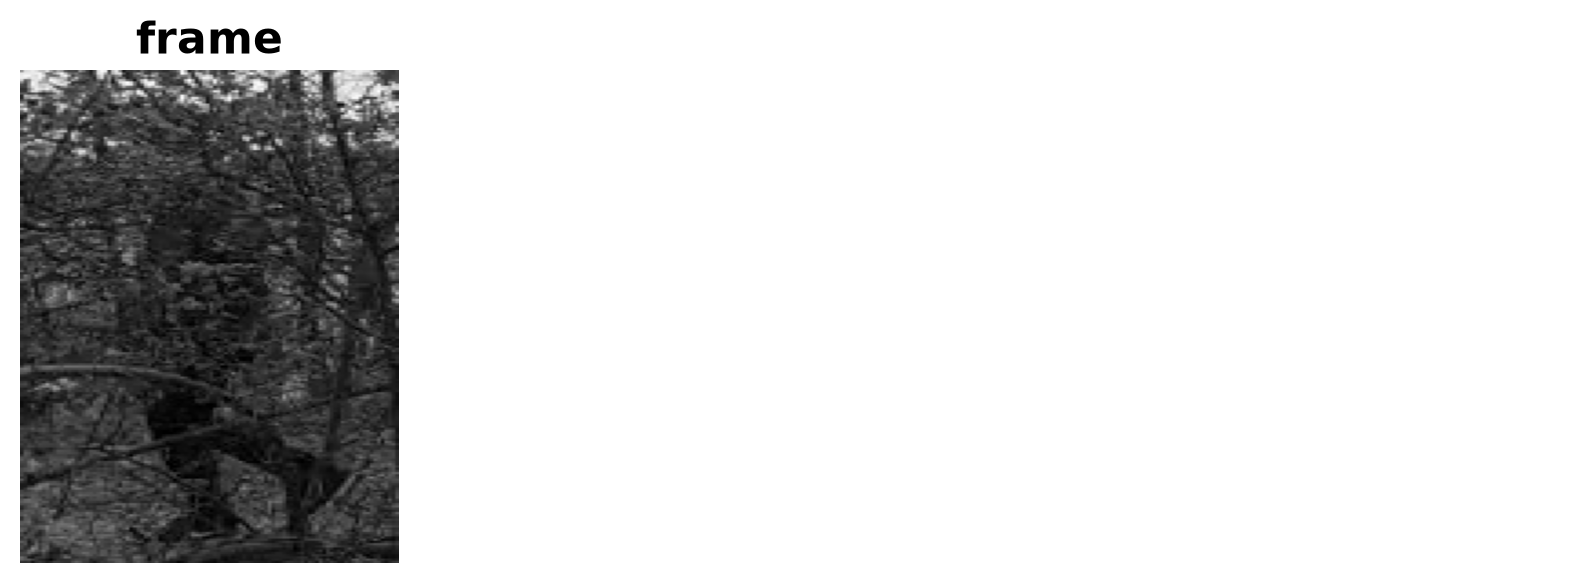
\includegraphics[width=0.86\textwidth]{plots/talk/annot_pair_q.png}\\[2mm]
\textbf{Which pixels are person?}}%
\only<2>{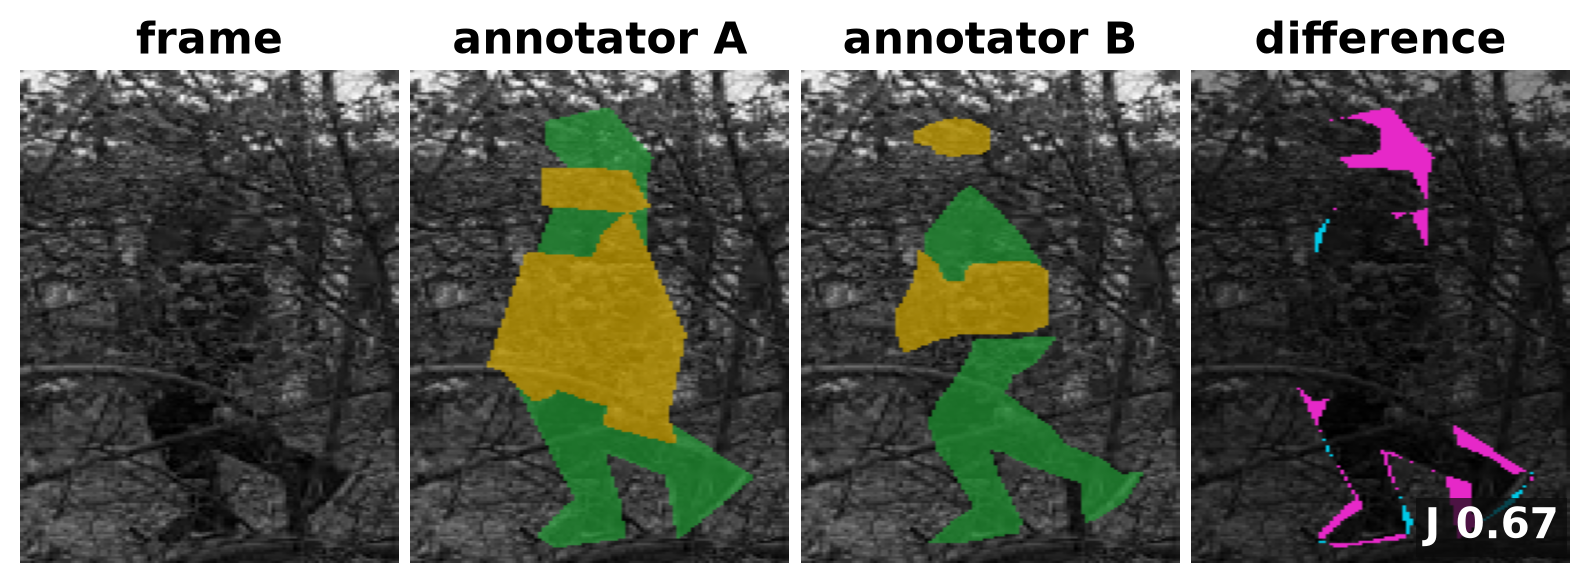
\includegraphics[width=0.86\textwidth]{plots/talk/annot_pair.png}\\[1mm]
\Klein{green: person,\ yellow: ambiguous;\quad difference: \textcolor{magenta}{\textbf{A only}}, \textcolor{cyan!70!blue}{\textbf{B only}}}\\[1mm]
$J = \dfrac{|A \cap B|}{|A \cup B|} \approx 0.65$ \quad \Klein{Jaccard index (IoU), ambiguous ignored}}
\note[itemize]{
\item Overlay 1: ask the room which pixels belong to the person. Overlay 2: two independent annotators.
\item J, the Jaccard index or intersection over union, is the standard segmentation score: 1 = identical, 0 = disjoint. Pixels marked ambiguous are left out.
\item Second annotator: independent, brush in CVAT, 15 frames of scenes 2 and 3. This frame is typical (median J 0.65).
\item They agree on the clear parts; they differ at the fragments, and in what they call ambiguous.
\item What a good label is depends on the annotator, and it takes long. The natural move: let a prompted model do it.
}
\end{frame}

\begin{frame}
\frametitle{Modal segmentation and ambiguous pixels}
\vspace*{2mm}
\begin{columns}[T]
\begin{column}{0.56\textwidth}
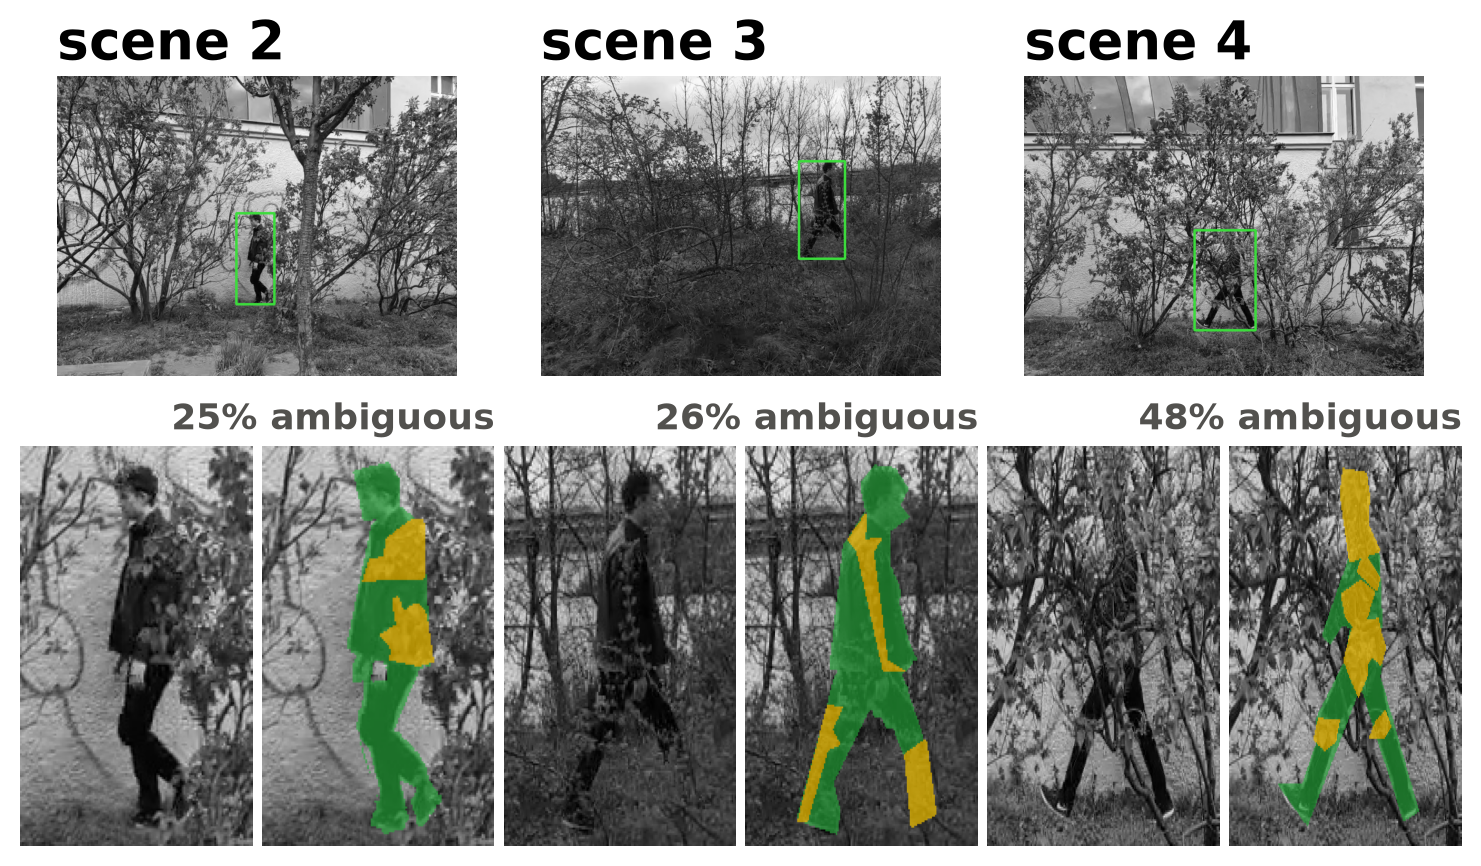
\includegraphics[width=\linewidth]{plots/talk/examples.png}
\end{column}
\begin{column}{0.42\textwidth}
\begin{itemize}
\item \textbf{modal}: the visible person; nothing invented behind the leaves
\item limited resolution, complex geometry: some pixels are ambiguous
\item ambiguous patches still hold person pixels
\item still useful for downstream tasks (tracking, detection)
\end{itemize}
\end{column}
\end{columns}
\note[itemize]{
\item Modal segmentation: the visible part. (Amodal would fill in the hidden body from a prior learnt on other images: hallucinated pixels, mixing the layers. We do not do that.)
\item Yellow: what the annotator marked ambiguous. On scenes 2--4 a median 0.21 of the person's box, as large as the visible part (0.22). These are not regions without a person; they are patches of person and leaf too fine to separate.
\item Including such a patch is partly wrong (the leaf pixels) and partly right (the person pixels). For tracking and detection the person pixels count more than the leaf pixels cost.
\item Same trade-off as in medical imaging: a missed lesion costs more than a false alarm, so the visible lesion gets a margin, but nothing is drawn where none was seen.
}
\end{frame}

\begin{frame}
\frametitle{PVS under fragmented occlusion}
\vspace*{2mm}
\begin{columns}[T]
\begin{column}{0.52\textwidth}
\centering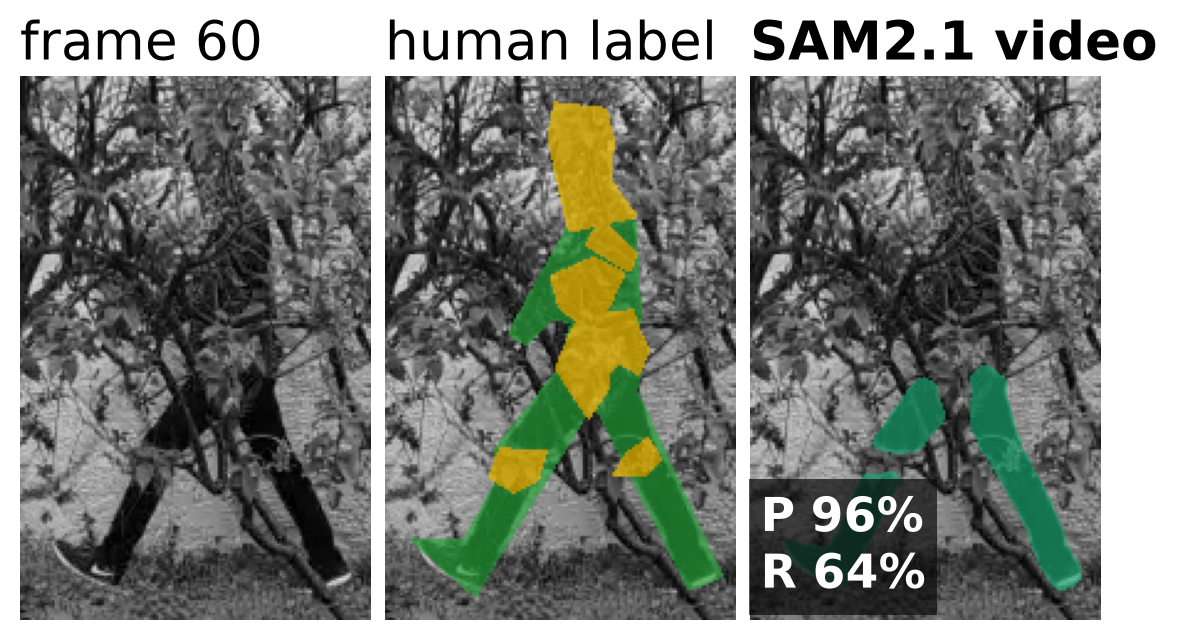
\includegraphics[width=\linewidth]{plots/talk/playsafe.png}
\end{column}
\begin{column}{0.46\textwidth}
\centering
\begin{tikzpicture}[node distance=7mm]
\node[sam] (s) {SAM2.1};
\node[box, left=6mm of s] (f) {frame $t$};
\node[box, right=6mm of s] (m) {mask $t$};
\node[box, below=9mm of s] (mem) {memory};
\draw[ar] (f) -- (s); \draw[ar] (s) -- (m);
\draw[ar] (m) |- (mem); \draw[ar] (mem) -- (s);
\end{tikzpicture}
\raggedright
\begin{itemize}
\item ambiguous pixels are left out
\item that mask goes into memory, and conditions the next
\item no clear frame to fall back on
\end{itemize}
\end{column}
\end{columns}
\note[itemize]{
\item SAM2.1 video, prompted once with box + point; frame 60 of a run in scene 4, against the human label.
\item Trained on clear objects, the model keeps only what it is sure about: the opposite of what we want here.
\item Memory is a closed loop: the next mask is conditioned on the cautious ones before it. Memory management (SAMURAI and others) chooses among past decisions; that helps when some past frame was clear. Here none is.
\item Expect the masks to shrink; the benchmark will show it.
}
\end{frame}

%=========================================================================================== III. benchmark
\Teil{The NFO-VOS benchmark}

\begin{frame}
\frametitle{The NFO dataset}
\centering
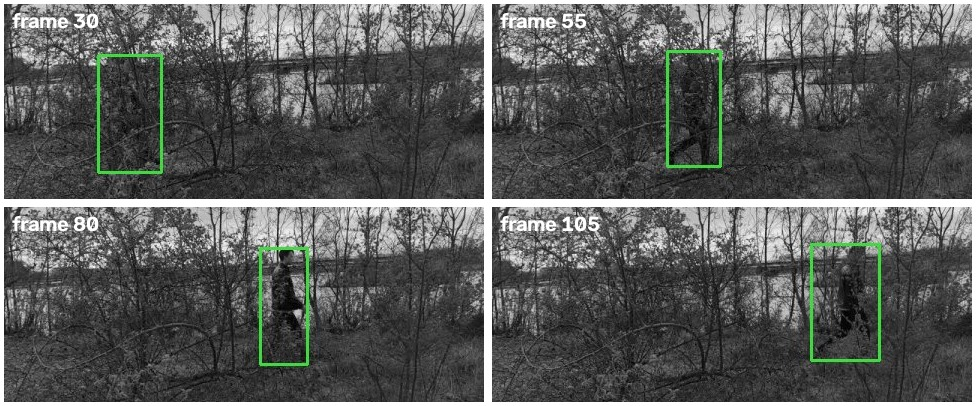
\includegraphics[height=5.2cm]{plots/talk/clip_strip.jpg}

\medskip\raggedright
\begin{itemize}
\item static camera, grayscale, $800\times600$; a person walks or runs across
\item a hand-drawn box in every frame; hand masks on 43 frames only
\item[$\Rightarrow$] score masks on tasks the boxes can check
\end{itemize}
\Quelle{NFO: Pflugfelder \& Auer, AVSS 2021}
\note[itemize]{
\item NFO (Pflugfelder \& Auer 2021): 4 scenes, fixed camera; per scene 8 runs (walk and run, left and right, each twice): 32 runs, 44--155 frames each; a hand-drawn person box in every frame. Made for person localisation.
\item One run (scene 3), four moments of the crossing, with the hand box. The full clip: plots/talk/clip.mp4.
\item NFO-VOS extends it into a segmentation benchmark. Hand masks: 43 frames, and two annotators agree only at J 0.65: not a basis for ranking methods. Boxes exist for every frame, so we score masks through tasks the boxes can check.
}
\end{frame}

\begin{frame}
\frametitle{Prompt placement}
\centering
\begin{tikzpicture}[x=2.1cm, y=0.85cm]
\pgfmathsetseed{7}
\foreach \i in {0,...,79} { \pgfmathsetmacro{\g}{20 + 70*rnd} \fill[TUMGruen!\g!white] (\i*0.12, 4.6) rectangle (\i*0.12 + 0.12, 5.3); }
\node[anchor=west, font=\PraesentationSchriftgroesseKlein\selectfont] at (9.7, 4.95) {foliage};
\foreach \y/\l/\d/\x in {3.6/{walk, right}/1/0.4, 2.6/{walk, left}/-1/6.9, 1.6/{run, right}/1/4.6, 0.6/{run, left}/-1/2.3} {
  \node[left, font=\PraesentationSchriftgroesseKlein\selectfont] at (0,\y) {\l};
  \ifnum\d=1 \draw[ar, black!25] (0.05,\y) -- (9.6,\y); \draw[ar, black!70, line width=1.2pt] (\x,\y) -- (9.6,\y);
  \else \draw[ar, black!25] (9.6,\y) -- (0.05,\y); \draw[ar, black!70, line width=1.2pt] (\x,\y) -- (0.05,\y); \fi
  \draw[densely dotted, black!50] (\x, \y) -- (\x, 4.6);
  \fill[black] (\x,\y) circle (3pt);
}
\end{tikzpicture}

\medskip\raggedright
\begin{itemize}
\item all runs of a scene pass the same foliage
\item each kind of run is prompted at a different offset $\to$ at a different visibility
\end{itemize}
\note[itemize]{
\item Shown: one run of each kind in one scene. Dot: where the prompt is given; dark: the part of the run that is segmented.
\item Visibility at the same position correlates r $\approx$ 0.65--0.73 between runs. So the runs are variations of one crossing, and we use them to sample the starting point: offsets 0, $\frac14$, $\frac12$, $\frac34$ of a 40-frame step. Twins start at the same offset.
\item Then we watch what happens over the rest of the run: we cannot assume the person is well visible when prompted.
}
\end{frame}

\begin{frame}
\frametitle{Evaluation: three downstream tasks}
\centering
\begin{tabular}{@{}c@{\hspace{12mm}}c@{\hspace{12mm}}c@{}}
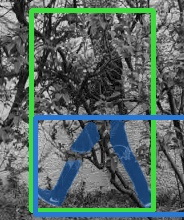
\includegraphics[height=4.4cm]{plots/nfo/bench_track.jpg} &
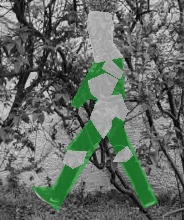
\includegraphics[height=4.4cm]{plots/nfo/bench_pixels.jpg} &
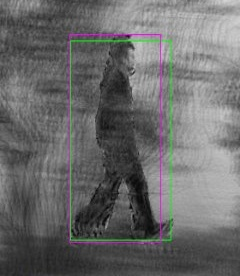
\includegraphics[height=4.4cm]{plots/nfo/bench_recog.jpg} \\[1mm]
\textbf{tracking} & \textbf{segmentation}$^{*}$ & \textbf{detection} \\
\Klein{box around the mask vs.\ hand box} & \Klein{J vs.\ hand masks} & \Klein{YOLO11 person detector}\\
\Klein{success AUC} & & \Klein{confidence, AP50}
\end{tabular}

\medskip\raggedright
\Klein{$^{*}$ experimental: 43 hand frames, two annotators. Reported for both, not used to rank.}
\note[itemize]{
\item Tracking: the box around the mask against the hand box, every frame; success rate over IoU thresholds, area under the curve (as in LaSOT).
\item Segmentation: J against the hand masks, ambiguous ignored. Shown for both annotators.
\item Detection: run the YOLO11 person detector on the image built from the masks (next slide). Confidence: score of the best detection overlapping the hand box (IoU $\ge$ 0.5). AP50: average precision at IoU 0.5 over all frames.
\item (Called \emph{recognition} on the poster and in the briefing; same metric.)
}
\end{frame}

\begin{frame}
\frametitle{Detection metric}
\vspace*{2mm}
\begin{columns}[T]
\begin{column}{0.44\textwidth}
\centering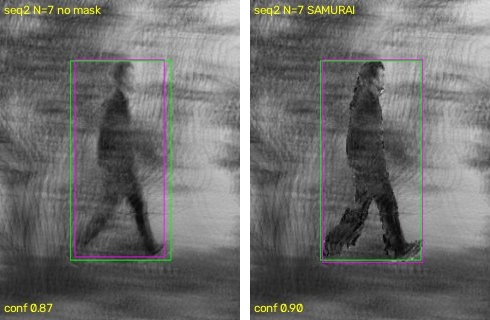
\includegraphics[width=\linewidth]{plots/talk/recog_plain_vs_masked.jpg}\\
\Klein{plain mean\hspace{20mm}masked mean}
\end{column}
\begin{column}{0.54\textwidth}
\begin{itemize}
\item shift the last $N = 5$ frames onto frame $t$ (hand-box motion, same for all methods)
\item average: foliage blurs, the person sharpens: the \textbf{integral image}
\item masked: average a pixel only over frames whose mask covers it
\item YOLO11 person detector on the result: \textbf{confidence} on the person, \textbf{AP50} over all frames
\end{itemize}
\end{column}
\end{columns}
\medskip
\Quelle{integral image: airborne optical sectioning, Kurmi, Schedl, Bimber 2021}
\note[itemize]{
\item This is the integral image of airborne optical sectioning: drone views of a forest registered on the ground and averaged, so the canopy blurs away and the ground comes into focus. Here the registration is on the moving person.
\item Masked mean: a pixel is averaged over the frames whose mask covers it; elsewhere the plain mean. Masked with SAM2.1 here. Example: $N = 7$, scene 2; the benchmark uses $N = 5$.
\item Confidence: score of the best person detection that overlaps the hand box (IoU $\ge$ 0.5), 0 if none. AP50: average precision of the person detections against the hand boxes, a hit at IoU $\ge$ 0.5, over all frames.
\item AP50: single frame 0.32, plain mean of 5 frames 0.66, masked 0.87.
}
\end{frame}

%=========================================================================================== IV. what Layer-SAM needs
\Teil{Where and what}

\begin{frame}
\frametitle{Mask size after a single prompt}
\vspace*{2mm}
\only<1>{%
\vspace*{2cm}\centering
{\PraesentationSchriftgroesseGross\selectfont Prompted once, with a perfect box.\\[3mm] 100 frames later, the mask is \dots\\[3mm] bigger \quad the same \quad smaller?}}%
\only<2>{%
\begin{columns}[T]
\begin{column}{0.62\textwidth}
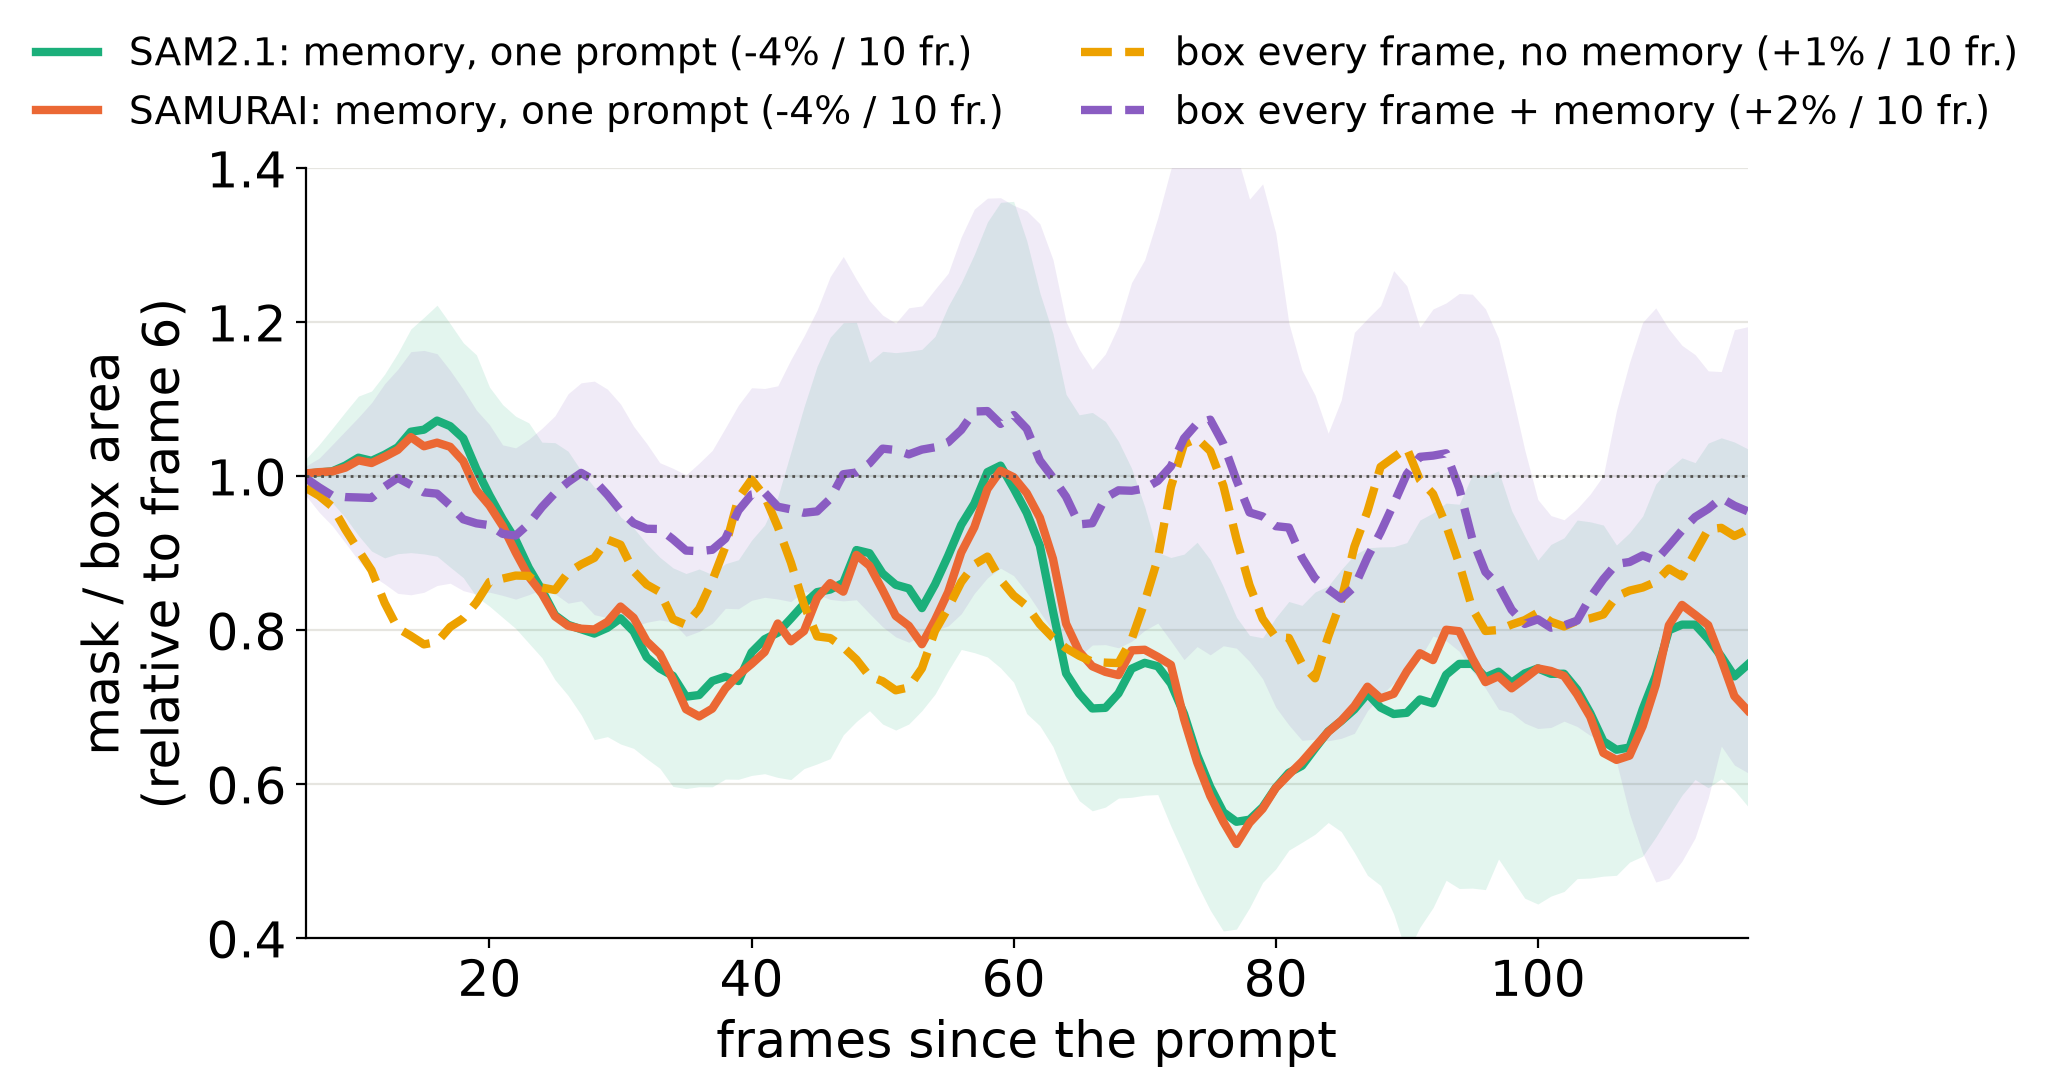
\includegraphics[width=\linewidth]{plots/talk/masksize_sam.png}
\end{column}
\begin{column}{0.36\textwidth}
\begin{itemize}
\item memory, one prompt: masks shrink
\item SAMURAI: the same
\item a box every frame: size kept
\item[$\Rightarrow$] we need a box every frame, without hand boxes
\end{itemize}
\end{column}
\end{columns}}
\note[itemize]{
\item Overlay 1: let the room guess first.
\item Mask area / box area relative to frame 6, median over the 32 runs, 95\,\% CI. SAM2.1 variants only.
\item Prompted once, memory masks shrink about 4\,\% per 10 frames: the cautious masks compound. SAMURAI's memory management changes nothing.
\item Telling SAM2.1 where to look in every frame (a box per frame, here from our tracker) keeps the size, with or without memory.
}
\end{frame}

\begin{frame}
\frametitle{Tracking vs.\ detection}
\centering
\begin{tabular}{@{}lcc@{}}
SAM2.1 & tracking AUC & detection conf \\\hline
memory, one prompt & .571 & \textbf{.666} \\
box every frame, no memory & .628 & .596 \\
box every frame + memory & \textbf{.661} & .636
\end{tabular}

\bigskip\raggedright
\begin{itemize}
\item a box every frame: the whole person, and foliage $\to$ tracking up, detection down
\item memory: what the person looks like $\to$ detection partly back
\item[$\Rightarrow$] we also need \emph{what} the person looks like, without a memory of masks
\end{itemize}
\note[itemize]{
\item A box every frame: tracking up (+0.057 without memory, +0.089 with), detection down: a box around a fragmented person holds foliage, and SAM2.1 takes some of it.
\item This is also why the benchmark has both tasks: tracking alone would reward boxes full of leaves, detection alone would reward caution.
\item So two things are needed: where (a box every frame) and what (evidence of the person's appearance). Both come from one idea: motion layers.
}
\end{frame}

\begin{frame}
\frametitle{Motion layers}
\centering\Schichten{1}

\bigskip
\raggedright
\begin{itemize}
\item static camera: foliage and background do not move
\item the person: approximately constant velocity $v$
\item align past frames at velocity $0$ $\to$ where; at $v$ $\to$ what
\end{itemize}
\Quelle{layers: Wang \& Adelson 1994}
\note[itemize]{
\item Wang \& Adelson (1994): describe a video as layers, each with its own motion, ordered in depth. Here: foliage in front, the person in the middle, the background behind.
\item Static camera: foliage and background move with velocity 0 (up to flutter). The person's motion is more complicated (gait, articulation); a constant horizontal velocity holds for people crossing a static camera's view at a distance: true for this data set.
\item Next two slides: one image per layer. Velocity 0 gives the empty scene, and from it a tracker (where). Velocity $v$ gives the integral image of the person (what).
}
\end{frame}

\begin{frame}
\frametitle{Empty scene and tracker}
\centering
\IfFileExists{plots/talk/changemap.png}{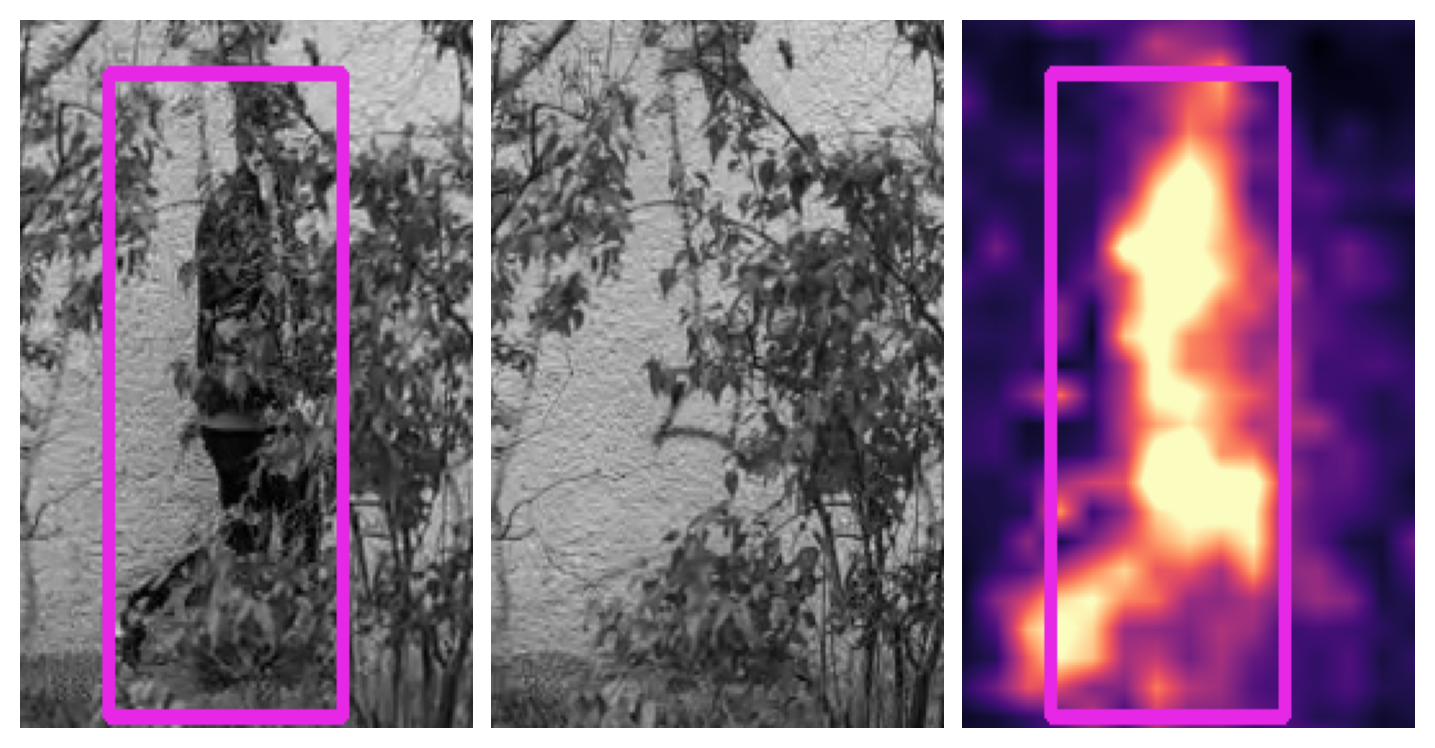
\includegraphics[height=4.4cm]{plots/talk/changemap.png}}{\Platzhalter{9cm}{4.6cm}{change map}}\\
\Klein{frame $t$ + tracker box\hspace{10mm}empty scene $B$\hspace{10mm}change $1 - \cos(F_t, F_B)$}

\medskip\raggedright
\begin{itemize}
\item empty scene $B$: median of frames without the person
\item change: how unlike $B$, per SAM2.1 feature cell
\item tracker: a fixed-size box moves to where change is largest, near a constant-velocity prediction
\end{itemize}
\note[itemize]{
\item Empty scene $B$: the static layers at velocity 0, a plain median of person-free frames. Encoded once by SAM2.1's encoder.
\item Change map: per feature cell, 1 minus the cosine similarity between frame $t$'s and the empty scene's features. The same idea as feature-based anomaly detection: distance to a ``normal'' reference in a pretrained feature space.
\item A box of the prompt's size slides over the change map near the predicted position (robust line fit through the last 8 positions) and moves to where the mean change is largest.
\item Shares the frame's encoder pass. Centre error 10 px on NFO. Where is solved; which pixels inside the box are person is not. The tracker also gives the person's velocity $v$: next slide.
}
\end{frame}

\begin{frame}
\frametitle{Integral image of the person}
\centering
\begin{tabular}{@{}c@{\hspace{10mm}}c@{\hspace{10mm}}c@{}}
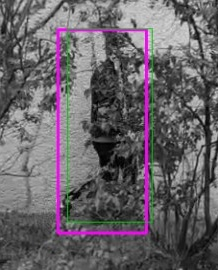
\includegraphics[height=5.0cm]{plots/nfo/inputs_0.jpg} &
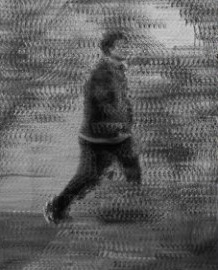
\includegraphics[height=5.0cm]{plots/nfo/inputs_2.jpg} &
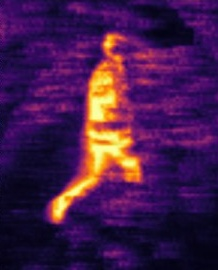
\includegraphics[height=5.0cm]{plots/nfo/inputs_3.jpg} \\
frame $t$ & integral image $C$ & evidence mass $a$
\end{tabular}

\medskip\raggedright
\begin{itemize}
\item the 6 frames before $t$, shifted by the tracker's velocity, averaged
\item as in the detection score, but with the tracker instead of hand boxes
\item same history as SAM2's memory: pixels, not masks
\item evidence mass $a$: how many past frames saw the person at each pixel
\end{itemize}
\note[itemize]{
\item Each past frame is shifted so the person lands where it is in frame $t$; averaged, the person adds up and the foliage blurs.
\item Two refinements, for the person layer only: recent frames weigh more (gait makes older frames drift); a pixel enters only where it clearly differs from the empty scene, so foliage does not pile up. The evidence mass $a$ is the weighted count of frames that entered at each pixel (bright: seen often, through gaps; dark: never seen, or only foliage). The adapter gets it as an extra input: it says where $C$ can be trusted.
\item 6 frames: the number of past frames SAM2 keeps in memory. Same history, but the pixels instead of the decisions.
\item Both images are the canonical images of a joint alignment of one layer; static camera and constant velocity make the alignment trivial.
}
\end{frame}

%=========================================================================================== V. Layer-SAM
\Teil{Layer-SAM}

\begin{frame}
\frametitle{Layer-SAM}
\centering\resizebox{!}{7.4cm}{% Layer-SAM, left to right, at slide size (the poster's plots/nfo/architecture.tex runs top to bottom).
% Colours as in the SAM2 paper figure: green encoder, orange decoder, lavender prompt encoder, pink memory (not used);
% blue outline = trained by us. Needs \Fire / \Ice (defined by plots/nfo/architecture.tex) and ColOurs / ColSamurai.
\definecolor{SamEnc}{HTML}{D4F5C4}\definecolor{SamEncD}{HTML}{8FCF79}
\definecolor{SamDec}{HTML}{FDE6C8}\definecolor{SamDecD}{HTML}{E9B676}
\definecolor{SamPrm}{HTML}{DEDDFB}\definecolor{SamPrmD}{HTML}{9E9BE6}
\definecolor{SamMem}{HTML}{F9DDF0}\definecolor{SamMemD}{HTML}{E7A9D3}
\begin{tikzpicture}[x=1cm, y=1cm, font=\PraesentationSchriftgroesseKlein\selectfont,
    a/.style={-{Latex[length=2.2mm]}, line width=0.9pt, draw=black!75},
    blk/.style={rounded corners=3pt, line width=0.9pt, align=center, inner sep=3pt},
    feat/.style={draw=SamEncD, fill=SamEnc!70, line width=0.7pt, minimum size=6.5mm, inner sep=0pt}]
  % inputs
  \foreach \n/\y/\f/\l in {X/2.5/inputs_0/{frame $t$\\{\color{black!60}tracker box}},
                           C/0/inputs_2/{integral image\\{\color{black!60}6 past frames}},
                           B/-2.5/inputs_1/{empty scene\\{\color{black!60}once per scene}}} {
    \node[inner sep=0pt] (\n) at (0, \y) {\includegraphics[height=2.1cm]{plots/nfo/\f.jpg}};
    \node[anchor=east, align=right] at (-1.0, \y) {\l};
  }
  % shared, frozen image encoder
  \node[blk, draw=SamEncD, fill=SamEnc, minimum width=1.1cm, minimum height=7.3cm] (enc) at (2.2, 0)
        {\rotatebox{90}{\Ice\ \textbf{image encoder}\ \ {\color{black!60}same weights for all three}}};
  \foreach \n/\y/\s in {X/2.5/t, C/0/C, B/-2.5/B} {
    \draw[a] (\n.east) -- (1.65, \y);
    \node[feat] (f\n) at (3.8, \y) {$F_{\s}$};
    \draw[a] (2.75, \y) -- (f\n.west);
  }
  % adapter
  \node[blk, draw=ColOurs, fill=ColOurs!12, line width=1.4pt, minimum width=2.5cm, minimum height=4.2cm] (ad) at (6.3, -1.25)
        {\Fire\ \textbf{adapter}\\0.7\,M\\[2mm]{\color{black!60}strides}\\{\color{black!60}16 $\to$ 8 $\to$ 4}};
  \draw[a] (fC.east) -- (fC.east -| ad.west);
  \draw[a] (fB.east) -- (fB.east -| ad.west);
  \draw[a] (5.5, 2.5) -- (5.5, 0.85);
  % corrected frame features
  \node[circle, draw=black!80, line width=1pt, minimum size=5.5mm, inner sep=0pt] (plus) at (8.6, 2.5) {$+$};
  \draw[a] (fX.east) -- (plus.west);
  \draw[a] (ad.east) -| node[pos=0.75, right] {$R$} (plus.south);
  % decoder, prompt encoder, tracker
  \node[blk, draw=SamDecD, fill=SamDec, minimum width=2.9cm, minimum height=9mm] (dec) at (11.2, 2.5) {\Ice\ \textbf{mask decoder}};
  \draw[a] (plus.east) -- node[above] {$\hat F_t$} (dec.west);
  \node[blk, draw=SamPrmD, fill=SamPrm, minimum width=2.9cm, minimum height=9mm] (pe) at (11.2, 0.3) {\Ice\ \textbf{prompt encoder}};
  \draw[a] (pe.north) -- (dec.south);
  \node[blk, draw=black!70, fill=white, line width=1.0pt, minimum width=2.9cm, minimum height=9mm] (trk) at (11.2, -2.0)
        {\textbf{tracker}\\{\color{black!60}box + point}};
  \draw[a] (trk.north) -- (pe.south);
  \draw[a, draw=black!45] (fB.south) -- (3.8, -3.75) -| node[pos=0.25, below, text=black!60] {change of $F_t$ against $F_B$} (trk.south);
  % output, memory not used, legend
  \node[inner sep=0pt] (M) at (14.4, 2.5) {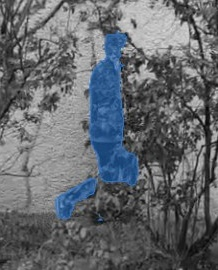
\includegraphics[height=2.1cm]{plots/nfo/inputs_6.jpg}};
  \draw[a] (dec.east) -- (M.west);
  \node[above=0.5mm of M] {mask};
  \node[blk, draw=SamMemD, fill=SamMem!50, dashed, text=black!55, minimum width=2.6cm] (mem) at (14.4, -0.4)
        {memory of\\past masks\\not used};
  \draw[a, draw=black!35, dashed] (M.south) -- node[text=ColSamurai, font=\large\bfseries, fill=white, inner sep=0pt] {$\times$} (mem.north);
  \node[align=left, anchor=north] at (14.4, -1.8) {\Fire\ trained\\\Ice\ frozen SAM2.1};
\end{tikzpicture}
}
\note[itemize]{
\item The tracker gives the prompt (where); the empty scene and the integral image are the two layers; frozen SAM2.1 decides once per frame.
\item Say: memory stores decisions; the integral image stores pixels. Memory stores masks that already threw the ambiguous pixels away; the integral image brings the information back every frame. No decision is fed back.
\item One frozen encoder for all three images; the empty scene once per scene: two encoder passes per frame. 61\,ms per frame vs 53\,ms for SAM2.1 video on a laptop GPU.
}
\end{frame}

\begin{frame}
\frametitle{Adapter architecture}
\centering
\resizebox{!}{5.6cm}{\begin{tikzpicture}[x=1cm, y=1cm, font=\PraesentationSchriftgroesseKlein\selectfont,
    lay/.style={draw=black!60, fill=black!5, rounded corners=2pt, line width=0.7pt, align=center, minimum height=9mm, inner sep=3pt},
    our/.style={lay, draw=ColOurs, fill=ColOurs!10}]
  \foreach \s/\y in {16/2.4, 8/0, 4/-2.4} {
    \node[lay, minimum width=3.4cm] (in\s) at (1.0, \y) {$F_t,\ F_C,\ F_B,\ a$\\{\color{black!60}stride \s}};
    \node[our] (p\s) at (4.3, \y) {$1{\times}1$ conv};
    \node[our, minimum width=5.0cm] (b\s) at (8.6, \y) {$2\times$ [$3{\times}3$ conv, GroupNorm, GELU]\\{\color{black!60}64 channels}};
    \node[our] (o\s) at (12.9, \y) {$1{\times}1$ conv\\{\color{black!60}zero init}};
    \node[circle, draw=black!80, inner sep=0pt, minimum size=5mm] (pl\s) at (14.6, \y) {$+$};
    \node[anchor=west] (r\s) at (15.0, \y) {$\hat F_t^{(\s)}$};
    \draw[ar] (in\s) -- (p\s); \draw[ar] (p\s) -- (b\s); \draw[ar] (b\s) -- (o\s); \draw[ar] (o\s) -- (pl\s);
    \draw[ar, black!50] (14.6, \y + 0.9) node[above] {$F_t^{(\s)}$} -- (pl\s);
  }
  \draw[ar] (b16.south) -- node[right] {upsample $\times 2$} (b8.north);
  \draw[ar] (b8.south) -- node[right] {upsample $\times 2$} (b4.north);
\end{tikzpicture}}

\medskip\raggedright
\begin{itemize}
\item inputs: features of frame, integral image, empty scene; evidence mass $a$ of the integral image
\item output: a correction to SAM2.1's features at each stride; an MLP shifts the tracker's point prompt
\item starts at zero: exactly SAM2.1 + tracker; 0.7\,M parameters, SAM2.1 frozen
\end{itemize}
\note[itemize]{
\item A decoder-style CNN over SAM2.1's multi-scale features, coarse (stride 16, 256 channels) to fine (stride 4, 32 channels).
\item At each stride: a shared $1{\times}1$ convolution projects the three feature maps; concatenated with the differences frame minus integral image and frame minus empty scene, and the evidence mass $a$ of the integral image (how many frames contributed per pixel).
\item Two $3{\times}3$ convolutions with GroupNorm and GELU; the coarser level's output is upsampled and concatenated into the next finer one.
\item A $1{\times}1$ output convolution, initialised to zero, maps back to SAM2.1's channels; its output is added to the frame's features. At step 0 the adapter adds nothing.
\item Point shift: a 2-layer MLP on the integral image's mean feature (weighted by evidence), zero-initialised last layer, added to the point token from the tracker.
\item 0.7\,M parameters in total. What it learns: where frame $t$ differs from the empty scene and agrees with the integral image, that is person evidence.
\item Training needs pixel-exact visible masks of people behind foliage. Nobody has them; we make them.
}
\end{frame}

\begin{frame}
\frametitle{Synthetic training data}
\vspace*{5mm}
\begin{columns}[T]
\begin{column}{0.2\textwidth}
\centering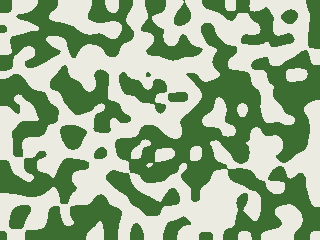
\includegraphics[height=2.5cm]{plots/talk/occluder_levelset.png}\\
\Klein{occlusion mask $A$}
\end{column}
\begin{column}{0.78\textwidth}
\begin{itemize}
\item a walking person, pasted into a forest photo
\item a random occlusion mask $A$: there, person pixels are replaced by the background
\item target, exact and free: the visible person $V = M \wedge \neg A$ \ \Klein{($M$: person mask)}
\end{itemize}
\end{column}
\end{columns}
\medskip
\centering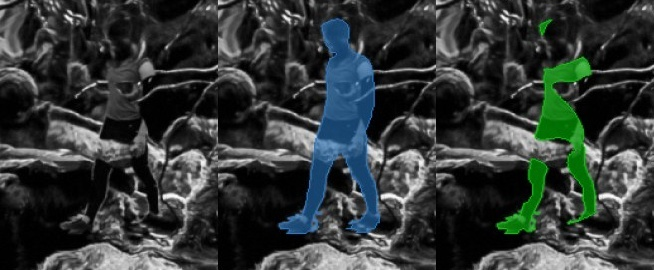
\includegraphics[width=0.36\textwidth]{plots/talk/synth_xmv.jpg}\\
\Klein{\makebox[0.12\textwidth]{frame}\makebox[0.12\textwidth]{$M$}\makebox[0.12\textwidth]{$V$}}\\
\raggedright
\Quelle{people: GPJATK, Kwolek et al.\ 2019;\ \ forests: CanaTree100, Grondin et al.\ 2023}
\note[itemize]{
\item Idea: the leaves are part of the forest photo; from a static camera leaves and background are one image. Where the occlusion mask is on, the photo is shown instead of the person, so the person appears behind the leaves. As a formula: frame $= A \cdot \text{photo} + (1 - A) \cdot (\text{person pasted into photo})$.
\item Occlusion mask: smooth random noise, thresholded to cover 20--60\,\% of pixels (leaf clumps of 12 or 24 px). Photo and mask sway together; NFO-calibrated sensor noise on top.
\item People: GPJATK gait sequences. Backgrounds: CanaTree100 or a foliage photo. Same tracker and integral image as at test time; clips generated on the fly.
}
\end{frame}

\begin{frame}
\frametitle{Loss function}
\vspace*{2mm}
\begin{columns}[T]
\begin{column}{0.26\textwidth}
\centering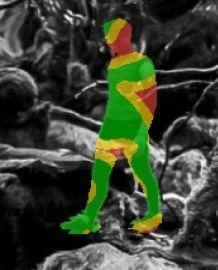
\includegraphics[height=5.4cm]{plots/talk/synth_w.jpg}\\
\Klein{weight: \textcolor{TUMGruen}{\textbf{1}}\ \ \textcolor[RGB]{230,184,0}{\textbf{0}}\ \ \textcolor{red!80!black}{\textbf{0.3}}}
\end{column}
\begin{column}{0.72\textwidth}
\begin{itemize}
\item from small-lesion segmentation in medicine: a miss costs more than a false alarm
\item Focal Tversky: $1 - \dfrac{TP}{TP + 0.3\,FP + 0.7\,FN}$ \ (+ per-pixel focal loss)
\item hidden, next to a visible fragment: \textbf{ignored}, the ambiguous band
\item hidden, far from any fragment: background, weight 0.3
\end{itemize}
\medskip
\Klein{AdamW, 200 steps of one fresh clip each; checkpoint chosen on scene 1 only; 3 seeds}\\
\Quelle{Focal Tversky: Abraham \& Khan 2019}
\end{column}
\end{columns}
\note[itemize]{
\item Same priority as on the ``modal segmentation'' slide. In lesion segmentation the target is small and scattered, and plain Dice under-weights misses; the Tversky index weights false negatives (0.7) above false positives (0.3). Focal: raised to 0.75, as in Abraham \& Khan.
\item Plus a per-pixel focal cross-entropy ($\gamma = 2$, person pixels weighted about 2:1), scaled by 20 as in SAM's recipe so the per-pixel term matters next to the overlap term.
\item Pixel weights: visible person and background 1; hidden person within 8 px of a visible fragment 0 (the annotators' ambiguous band, yellow); hidden person far from any fragment 0.3, counted as background: modal, but not harshly.
\item AdamW, learning rate $3\cdot10^{-4}$, weight decay $10^{-4}$, cosine schedule; up to 32 target frames per clip. Checkpoint at step 200, chosen on scene 1; scenes 2--4 are the test.
\item Rejected: a precision-leaning focal default (recall 0.76 $\rightarrow$ 0.61), a balanced loss (J $-$0.026 on scenes 2--4).
}
\end{frame}

%=========================================================================================== VI. results
\Teil{Results}

\begin{frame}
\frametitle{Qualitative comparison}
\vspace*{4mm}\centering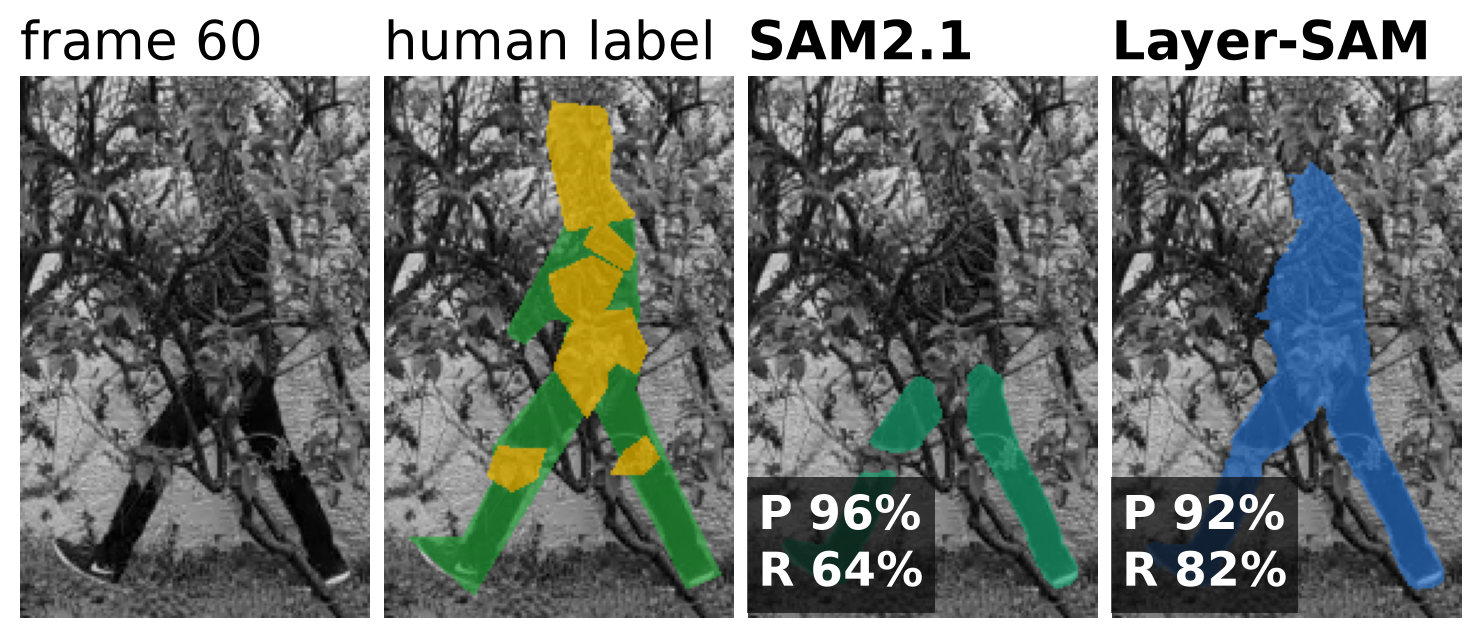
\includegraphics[height=6.4cm]{plots/talk/qual1.png}
\note[itemize]{
\item The frame from the ``PVS under fragmented occlusion'' slide again (scene 4, frame 60), against the human label; precision P and recall R in the corners.
\item SAM2.1 keeps the clearest fragments; Layer-SAM marks the fragments the annotator marked, at a small cost in precision.
}
\end{frame}

\begin{frame}
\frametitle{Results on NFO-VOS}
\centering
\setlength{\tabcolsep}{6pt}
\resizebox{0.85\textwidth}{!}{%
\begin{tabular}{@{}l c cc cc@{}}
 & \textbf{tracking} & \multicolumn{2}{c}{\textbf{segmentation}$^{*}$} & \multicolumn{2}{c}{\textbf{detection}} \\
 & AUC & J$_A$ & J$_B$ & conf & AP50 \\\hline
SAM2.1 (memory) & .571 & .733 & \textbf{.657} & .666 & .869 \\
SAMURAI & .579 & .730 & .647 & .663 & .863 \\
SAM2.1 + tracker box + memory & .661 & .745 & .614 & .636 & .861 \\
SAM2.1 + tracker box & .628 & .685 & .588 & .596 & .814 \\
\color{ColOurs}\textbf{Layer-SAM (no memory)} & \color{ColOurs}\textbf{.678} & \color{ColOurs}\textbf{.756} & \color{ColOurs}.649 & \color{ColOurs}\textbf{.667} & \color{ColOurs}\textbf{.878}
\end{tabular}}

\medskip\raggedright
\begin{itemize}
\item no memory at all: best tracking, +0.10 AUC vs.\ SAMURAI (all 95\,\% CIs $> 0$)
\item segmentation$^{*}$: +0.02--0.03 $J_A$ vs.\ SAMURAI (all CIs $> 0$); on par in $J_B$
\item detection: on par in confidence, highest AP50
\item cost: 61\,ms per frame vs.\ 53\,ms for SAM2.1 with memory (+15\,\%, laptop GPU)
\end{itemize}
\Klein{32 runs, 4 scenes; Layer-SAM: mean of 3 seeds. $^{*}$ A: 43 frames (scenes 1--4), B: 15 frames (scenes 2, 3).}
\note[itemize]{
\item Tracking: Layer-SAM vs SAMURAI +0.096 to +0.102 AUC per seed, every paired bootstrap CI above 0; also ahead of SAM2.1 with memory and a box every frame.
\item CIs: paired window bootstrap per seed vs SAMURAI (resampling runs/clips). Segmentation, annotator A: +0.022 to +0.029 J per seed, every CI above 0; the gain is recall (0.86 vs 0.81) at slightly lower precision (0.86 vs 0.88). Annotator B: 15 frames, no CI; 0.649 vs 0.647 SAMURAI, 0.657 SAM2.1: on par.
\item Detection confidence vs SAMURAI: $-$0.001 to +0.008 per seed: on par. AP50 0.878 is the highest in the table, but no CI was computed for it.
\item The point: Layer-SAM uses no memory whatsoever; integrated pixels carry what memory would carry, without compounding caution.
\item Cost: one shared encoder pass per frame for the frame and one for the integral image (the empty scene once per scene); tracker and adapter are small. 61\,ms vs 53\,ms per frame for SAM2.1 video, RTX PRO 4000 laptop GPU, batch 1.
}
\end{frame}

\begin{frame}
\frametitle{Ablation}
\vspace*{2mm}
\begin{columns}[T]
\begin{column}{0.64\textwidth}
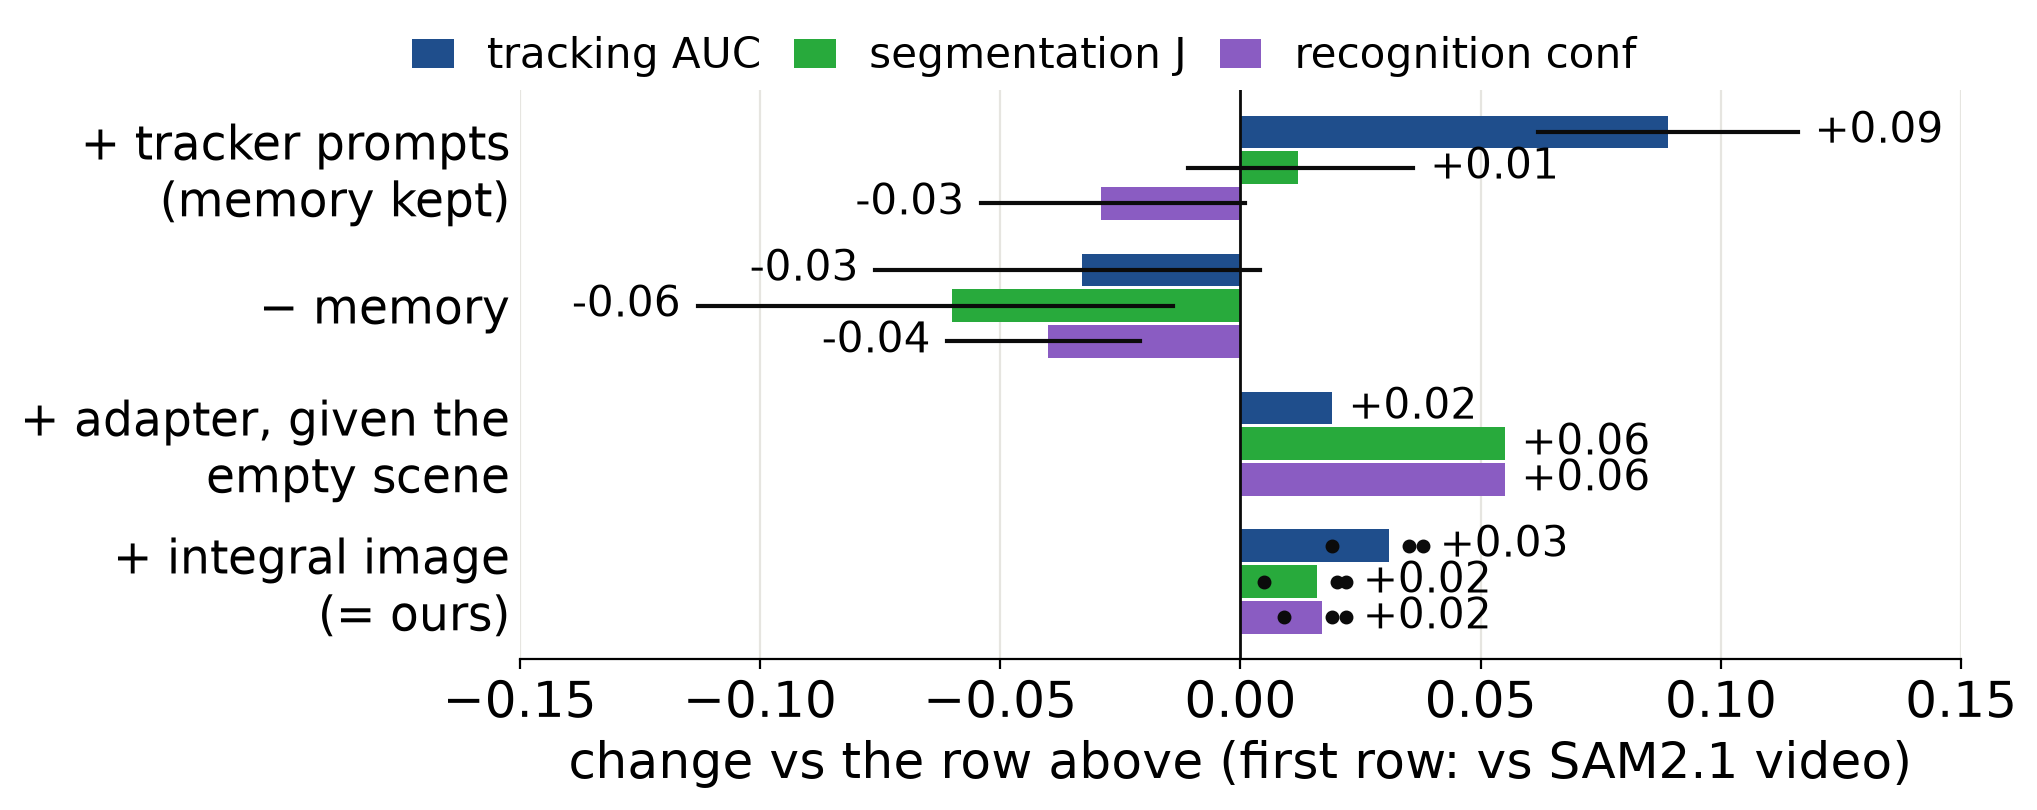
\includegraphics[width=\linewidth]{plots/nfo/ablation.png}
\end{column}
\begin{column}{0.34\textwidth}
\begin{itemize}
\item tracker: where
\item empty scene: precision
\item integral image: recall
\end{itemize}
\end{column}
\end{columns}
\note[itemize]{
\item From SAM2.1 video to Layer-SAM, one change per row (J here: annotator A, all 43 frames).
\item Tracker prompts: tracking up, precision down. Removing memory: everything down.
\item Adapter with the empty scene only: precision 0.80 $\rightarrow$ 0.88.
\item Integral image: recall 0.81 $\rightarrow$ 0.85; tracking +0.019 to +0.038 and detection +0.009 to +0.022 per seed.
}
\end{frame}

\begin{frame}
\frametitle{Detection vs.\ number of integrated frames}
\vspace*{2mm}
\begin{columns}[T]
\begin{column}{0.58\textwidth}
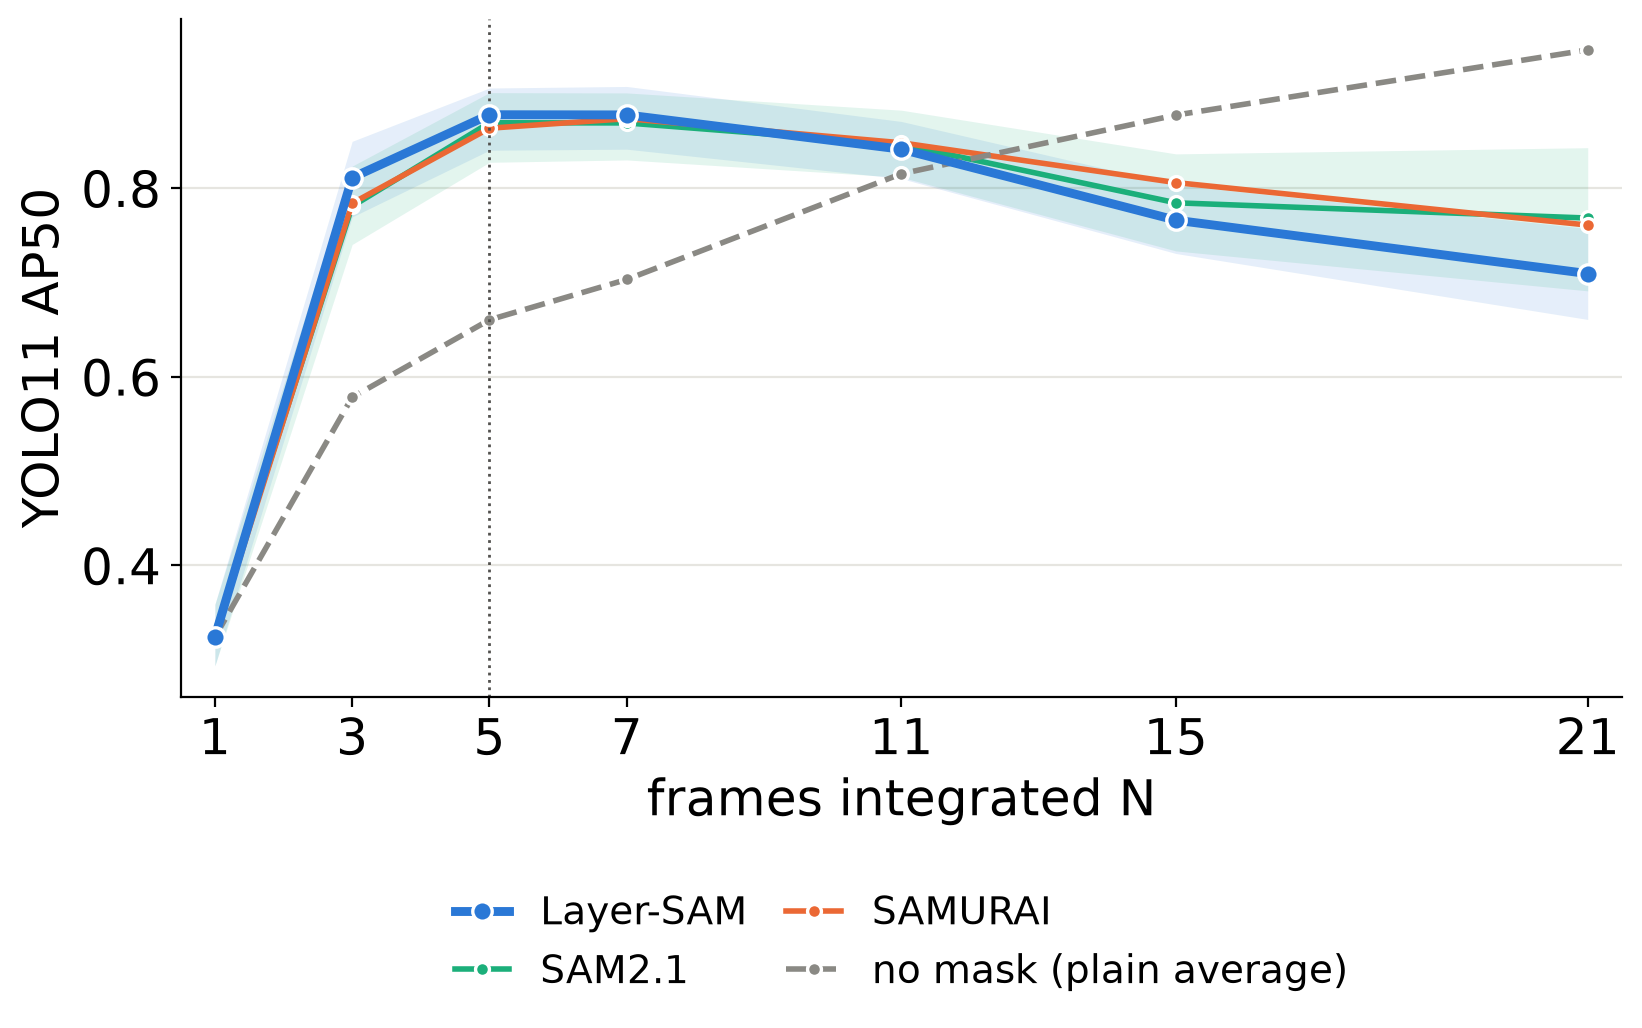
\includegraphics[width=\linewidth]{plots/talk/recogN4.png}
\end{column}
\begin{column}{0.4\textwidth}
\begin{itemize}
\item one frame: AP50 .32; three frames: about .8
\item Layer-SAM best up to $N = 7$; the benchmark uses 5
\item many frames: the plain mean wins, masks only add their errors
\end{itemize}
\end{column}
\end{columns}
\note[itemize]{
\item YOLO11 AP50 vs the number of integrated frames $N$, 32 runs (Layer-SAM: one seed).
\item Integration is what makes detection work. $N = 5$ is where SAM2.1 and SAMURAI score best: the fair choice for the baselines.
\item At 3 frames Layer-SAM leads (0.81 vs 0.78); at long $N$ it falls below SAM2.1 (0.71 vs 0.77 at 21), probably its lower precision: any foliage its masks include is averaged in.
\item From $N$ 11 the plain mean wins outright (0.95 at 21): with true motion and enough frames, no mask is needed.
}
\end{frame}

%=========================================================================================== VII. conclusion
\Teil{Conclusion}

\begin{frame}
\frametitle{Conclusion}
\begin{enumerate}
\item behind foliage: never a full view; some pixels stay ambiguous
\item downstream tasks want them; PVS drops them, and memory compounds it
\item motion layers: the empty scene says where, the integral image says what
\item Layer-SAM, no memory: best tracking, on par elsewhere
\end{enumerate}
\medskip
\Merke{When each decision drops evidence, aggregate the evidence first, then decide.}
\note[itemize]{
\item A static wall of leaves in front of a moving person: no frame shows all of it, not at the prompt, not later. Some patches mix person and leaf too finely to resolve, for any model and for annotators (J 0.65).
\item For tracking and detection, the person pixels in such patches are worth more than the leaf pixels cost. A PVS model leaves them out, stores that mask, and conditions the next one on it: the masks shrink.
\item What we know about the scene (static camera, moving person) separates it into layers by motion; their images accumulate evidence, and deciding once per frame from them, without memory, works better.
}
\end{frame}

\begin{frame}
\frametitle{Open questions}
\begin{itemize}
\item moving camera, articulated motion: \textbf{joint alignment} of all layers
\item integral image in \textbf{feature space}: one encoder pass?
\item other use cases: distractors, other occluders, by motion layers?
\end{itemize}
\note[itemize]{
\item A moving camera turns the empty scene into a registered background layer; articulation needs more than one shift per frame. Estimate all layer motions together, with occlusion modelled so static leaves do not bias the registration.
\item Feature space: averaging features is not encoding the average (the encoder is non-linear), and a feature cell is larger than most gaps. Whether a clean integral image exists there is open.
\item A look-alike person moves differently, so a motion layer can separate it; other fragmented occluders (fences, blinds, rain).
}
\end{frame}

\begin{frame}
\frametitle{References}
{\fontsize{9}{11.5}\selectfont
Pflugfelder, Auer (2021). Person localisation under fragmented occlusion. AVSS.\\
Ravi et al.\ (2024). SAM 2: segment anything in images and videos. arXiv 2408.00714.\\
Yang et al.\ (2024). SAMURAI. arXiv 2411.11922.\\
Kurmi, Schedl, Bimber (2021, 2022). Airborne optical sectioning. arXiv 2111.06959, 2207.13344.\\
Wang, Adelson (1994). Representing moving images with layers. IEEE TIP.\\
Abraham, Khan (2019). A novel focal Tversky loss function. ISBI.\\
Jocher et al.\ (2024). Ultralytics YOLO11.\\
Kwolek et al.\ (2019). Calibrated and synchronized multi-view video and motion capture dataset for evaluation of gait recognition (GPJATK). Multimedia Tools and Applications.\\
Grondin et al.\ (2023). Tree detection and diameter estimation based on deep learning (CanaTree100). Forestry.\\
Perazzi et al.\ (2016). A benchmark dataset and evaluation methodology for video object segmentation (DAVIS). CVPR.\\
Image source (DAVIS strip): to fill in.\par}
\end{frame}

\begin{frame}[plain]
\centering
\vspace*{3.2cm}
{\PraesentationSchriftgroesseSehrGross\selectfont Thank you}

\bigskip
ido.akov@tum.de
\end{frame}

\end{document} % !!! NICHT ENTFERNEN !!!
